%%%%%%%%%%%%%%%%%%%%%%%%%%%%%%%%%%%%%%%%%
%  A bright and image filled report style, currently set up here for use with ILM report 8600-219.
%  Contains all that is required, glossaries, content management, references and good looks.
%
% The original template (the Legrand Orange Book Template) can be found here --> http://www.latextemplates.com/template/the-legrand-orange-book
% Original author of the Legrand Orange Book Template:
% Mathias Legrand (legrand.mathias@gmail.com) 
%
% Modifications made for ILM specific reporting
% 
%
% License:
% CC BY-NC-SA 3.0 (http://creativecommons.org/licenses/by-nc-sa/3.0/)
%%%%%%%%%%%%%%%%%%%%%%%%%%%%%%%%%%%%%%%%%
 
%%%%%%%%%%%%%%%%%%%%%%%%%%%%%%%%%%%%%%%%%
% How to use this
%
% Upload a file called FrontCover.jpg to become your new front cover - into the Pictures folder
% Upload files called Heading1.jpg, Heading2.jpg etc to become your new chapter headers - into the Pictures folder
% Make sure these images are the right size to fit their locations and use good quality images
%
% Locate the variables below and set your name, title etc.
%
% If you want to change text colour on the front cover, the areas required are commented below
% If you want to modify text and border colours for your chapter headers go into the structure.tex file and replace the name of the colour (set to ) with a new colour name (find and replace ctrl+f will do this for you).
%
% Add all references into references.bib
% Cite these references by using \cite{referenceName}
%
% Commonly used acronyms or industry specific terms should be added to the glossary
% These terms may then be referenced in the text using \gls{termName}
%
% Finally put some answers in there!
%
% 
% Note: This template is set up specifically for ILM reports, it can be modified for other forms of reports
%
%%%%%%%%%%%%%%%%%%%%%%%%%%%%%%%%%%%%%%%%
 
 
%----------------------------------------------------------------------------------------
%	SET THESE VARIABLES!
%----------------------------------------------------------------------------------------

\def\mytitle{ Vectorial Calculus } % Title of the ILM project
\def\ILMCode{Adbridged, it seems.} % Unique code for the ILM project

\def\author{Jaime Andres Torres B.} % Your name.. 
\def\id{github.com/XaurDesu} % Your unique identifier

\def\date{\today } % Today's date 


 
%----------------------------------------------------------------------------------------
%	PACKAGES AND OTHER DOCUMENT CONFIGURATIONS
%----------------------------------------------------------------------------------------

\documentclass[11pt,fleqn]{book} % Default font size and left-justified equations

\usepackage[dvipsnames]{xcolor}

%%%%%%%%%%%%%%%%%%%%%%%%%%%%%%%%%%%%%%%%%
% This is based on the Legrand Orange Book
% Structural Definitions File
%
% The original template (the Legrand Orange Book Template) can be found here --> http://www.latextemplates.com/template/the-legrand-orange-book
%
% Original author of the Legrand Orange Book Template::
% Mathias Legrand (legrand.mathias@gmail.com) with modifications by:
% Vel (vel@latextemplates.com)
%
% Original License:
% CC BY-NC-SA 3.0 (http://creativecommons.org/licenses/by-nc-sa/3.0/)
%
%%%%%%%%%%%%%%%%%%%%%%%%%%%%%%%%%%%%%%%%%
%----------------------------------------------------------------------------------------
%	VARIOUS REQUIRED PACKAGES
%----------------------------------------------------------------------------------------

\usepackage{titlesec} % Allows customization of titles

\usepackage{graphicx} % Required for including pictures
\graphicspath{{Pictures/}} % Specifies the directory where pictures are stored

\usepackage{lipsum} % Inserts dummy text

\usepackage{tikz} % Required for drawing custom shapes

\usepackage[english]{babel} % English language/hyphenation

\usepackage{enumitem} % Customize lists

\setlist{nolistsep} % Reduce spacing between bullet points and numbered lists

\usepackage{booktabs} % Required for nicer horizontal rules in tables

\usepackage{eso-pic} % Required for specifying an image background in the title page

\usepackage{glossaries} %Required to allow the creation of glossary items, allows for referencing within the document

\usepackage[none]{hyphenat} %Stops words which are too long for a line being split over two lines using hyphenation

\usepackage[top=3cm,bottom=3cm,left=3.2cm,right=3.2cm,headsep=10pt,letterpaper]{geometry} % Page margins
\usepackage{algorithm} % Writing nice algorithms
\usepackage{algpseudocode} % Writing pseudocode
\usepackage{longtable} %Tables which may stretch over more than 1 page
\usepackage{rotating} %Rotate images using sideswaysimage


% Font Settings
\usepackage{avant} % Use the Avantgarde font for headings
%\usepackage{times} % Use the Times font for headings
\usepackage{mathptmx} % Use the Adobe Times Roman as the default text font together with math symbols from the Symbol, Chancery and Computer Modern fonts

\usepackage{microtype} % Slightly tweak font spacing for aesthetics
\usepackage[utf8]{inputenc} % Required for including letters with accents
\usepackage[T1]{fontenc} % Use 8-bit encoding that has 256 glyphs

%----------------------------------------------------------------------------------------
%	MAIN TABLE OF CONTENTS
%----------------------------------------------------------------------------------------

\usepackage{titletoc} % Required for manipulating the table of contents

\contentsmargin{0cm} % Removes the default margin
% Chapter text styling
\titlecontents{chapter}[1.25cm] % Indentation
{\addvspace{15pt}\large\sffamily\bfseries} % Spacing and font options for chapters
{\color{Apricot!60}\contentslabel[\Large\thecontentslabel]{1.25cm}\color{Apricot}} % Chapter number
{}  
{\color{Apricot!60}\normalsize\sffamily\bfseries\;\titlerule*[.5pc]{.}\;\thecontentspage} % Page number
% Section text styling
\titlecontents{section}[1.25cm] % Indentation
{\addvspace{5pt}\sffamily\bfseries} % Spacing and font options for sections
{\contentslabel[\thecontentslabel]{1.25cm}} % Section number
{}
{\sffamily\hfill\color{black}\thecontentspage} % Page number
[]
% Subsection text styling
\titlecontents{subsection}[1.25cm] % Indentation
{\addvspace{1pt}\sffamily\small} % Spacing and font options for subsections
{\contentslabel[\thecontentslabel]{1.25cm}} % Subsection number
{}
{\sffamily\;\titlerule*[.5pc]{.}\;\thecontentspage} % Page number
[] 

%----------------------------------------------------------------------------------------
%	MINI TABLE OF CONTENTS IN CHAPTER HEADS
%----------------------------------------------------------------------------------------

% Section text styling
\titlecontents{lsection}[0em] % Indendating
{\footnotesize\sffamily} % Font settings
{}
{}
{}

% Subsection text styling
\titlecontents{lsubsection}[.5em] % Indentation
{\normalfont\footnotesize\sffamily} % Font settings
{}
{}
{}
 
%----------------------------------------------------------------------------------------
%	PAGE HEADERS
%----------------------------------------------------------------------------------------

\usepackage{fancyhdr} % Required for header and footer configuration

\pagestyle{fancy}
\renewcommand{\chaptermark}[1]{\markboth{\sffamily\normalsize\bfseries\chaptername\ \thechapter.\ #1}{}} % Chapter text font settings
\renewcommand{\sectionmark}[1]{\markright{\sffamily\normalsize\thesection\hspace{5pt}#1}{}} % Section text font settings
\fancyhf{} \fancyhead[LE,RO]{\sffamily\normalsize\thepage} % Font setting for the page number in the header
\fancyhead[LO]{\rightmark} % Print the nearest section name on the left side of odd pages
\fancyhead[RE]{\leftmark} % Print the current chapter name on the right side of even pages
\renewcommand{\headrulewidth}{0.5pt} % Width of the rule under the header
\addtolength{\headheight}{2.5pt} % Increase the spacing around the header slightly
\renewcommand{\footrulewidth}{0pt} % Removes the rule in the footer
\fancypagestyle{plain}{\fancyhead{}\renewcommand{\headrulewidth}{0pt}} % Style for when a plain pagestyle is specified

% Removes the header from odd empty pages at the end of chapters
\makeatletter
\renewcommand{\cleardoublepage}{
\clearpage\ifodd\c@page\else
\hbox{}
\vspace*{\fill}
\thispagestyle{empty}
\newpage
\fi}

%----------------------------------------------------------------------------------------
%	THEOREM STYLES
%----------------------------------------------------------------------------------------

\usepackage{amsmath,amsfonts,amssymb,amsthm} % For math equations, theorems, symbols, etc

\newcommand{\intoo}[2]{\mathopen{]}#1\,;#2\mathclose{[}}
\newcommand{\ud}{\mathop{\mathrm{{}d}}\mathopen{}}
\newcommand{\intff}[2]{\mathopen{[}#1\,;#2\mathclose{]}}
\newtheorem{notation}{Notation}[chapter]

%%%%%%%%%%%%%%%%%%%%%%%%%%%%%%%%%%%%%%%%%%%%%%%%%%%%%%%%%%%%%%%%%%%%%%%%%%%
%%%%%%%%%%%%%%%%%%%% dedicated to boxed/framed environements %%%%%%%%%%%%%%
%%%%%%%%%%%%%%%%%%%%%%%%%%%%%%%%%%%%%%%%%%%%%%%%%%%%%%%%%%%%%%%%%%%%%%%%%%%
\newtheoremstyle{Orchidnumbox}% % Theorem style name
{0pt}% Space above
{0pt}% Space below
{\normalfont}% % Body font
{}% Indent amount
{\small\bf\sffamily\color{Apricot}}% % Theorem head font
{\;}% Punctuation after theorem head
{0.25em}% Space after theorem head
{\small\sffamily\color{Apricot}\thmname{#1}\nobreakspace\thmnumber{\@ifnotempty{#1}{}\@upn{#2}}% Theorem text (e.g. Theorem 2.1)
\thmnote{\nobreakspace\the\thm@notefont\sffamily\bfseries\color{black}---\nobreakspace#3.}} % Optional theorem note
\renewcommand{\qedsymbol}{$\blacksquare$}% Optional qed square

\newtheoremstyle{blacknumex}% Theorem style name
{5pt}% Space above
{5pt}% Space below
{\normalfont}% Body font
{} % Indent amount
{\small\bf\sffamily}% Theorem head font
{\;}% Punctuation after theorem head
{0.25em}% Space after theorem head
{\small\sffamily{\tiny\ensuremath{\blacksquare}}\nobreakspace\thmname{#1}\nobreakspace\thmnumber{\@ifnotempty{#1}{}\@upn{#2}}% Theorem text (e.g. Theorem 2.1)
\thmnote{\nobreakspace\the\thm@notefont\sffamily\bfseries---\nobreakspace#3.}}% Optional theorem note

\newtheoremstyle{blacknumbox} % Theorem style name
{0pt}% Space above
{0pt}% Space below
{\normalfont}% Body font
{}% Indent amount
{\small\bf\sffamily}% Theorem head font
{\;}% Punctuation after theorem head
{0.25em}% Space after theorem head
{\small\sffamily\thmname{#1}\nobreakspace\thmnumber{\@ifnotempty{#1}{}\@upn{#2}}% Theorem text (e.g. Theorem 2.1)
\thmnote{\nobreakspace\the\thm@notefont\sffamily\bfseries---\nobreakspace#3.}}% Optional theorem note

%%%%%%%%%%%%%%%%%%%%%%%%%%%%%%%%%%%%%%%%%%%%%%%%%%%%%%%%%%%%%%%%%%%%%%%%%%%
%%%%%%%%%%%%% dedicated to non-boxed/non-framed environements %%%%%%%%%%%%%
%%%%%%%%%%%%%%%%%%%%%%%%%%%%%%%%%%%%%%%%%%%%%%%%%%%%%%%%%%%%%%%%%%%%%%%%%%%
\newtheoremstyle{Orchidnum}% % Theorem style name
{5pt}% Space above
{5pt}% Space below
{\normalfont}% % Body font
{}% Indent amount
{\small\bf\sffamily\color{Apricot}}% % Theorem head font
{\;}% Punctuation after theorem head
{0.25em}% Space after theorem head
{\small\sffamily\color{Apricot}\thmname{#1}\nobreakspace\thmnumber{\@ifnotempty{#1}{}\@upn{#2}}% Theorem text (e.g. Theorem 2.1)
\thmnote{\nobreakspace\the\thm@notefont\sffamily\bfseries\color{black}---\nobreakspace#3.}} % Optional theorem note
\renewcommand{\qedsymbol}{$\blacksquare$}% Optional qed square
\makeatother

% Defines the theorem text style for each type of theorem to one of the three styles above
\newcounter{dummy} 
\numberwithin{dummy}{section}
\theoremstyle{Orchidnumbox}
\newtheorem{theoremeT}[dummy]{Theorem}
\newtheorem{problem}{Problem}[chapter]
\newtheorem{exerciseT}{Exercise}[chapter]
\theoremstyle{blacknumex}
\newtheorem{exampleT}{Example}[chapter]
\theoremstyle{blacknumbox}
\newtheorem{vocabulary}{Vocabulary}[chapter]
\newtheorem{definitionT}{Definition}[section]
\newtheorem{corollaryT}[dummy]{Corollary}
\theoremstyle{Orchidnum}
\newtheorem{proposition}[dummy]{Proposition}

%----------------------------------------------------------------------------------------
%	DEFINITION OF COLORED BOXES
%----------------------------------------------------------------------------------------

\RequirePackage[framemethod=default]{mdframed} % Required for creating the theorem, definition, exercise and corollary boxes

% Theorem box
\newmdenv[skipabove=7pt,
skipbelow=7pt,
backgroundcolor=black!5,
linecolor= Apricot, % Modify the colour of theorem boxes
innerleftmargin=5pt,
innerrightmargin=5pt,
innertopmargin=5pt,
leftmargin=0cm,
rightmargin=0cm,
innerbottommargin=5pt]{tBox}

% Exercise box	  
\newmdenv[skipabove=7pt,
skipbelow=7pt,
rightline=false,
leftline=true,
topline=false,
bottomline=false,
backgroundcolor=Apricot!10,
linecolor=Apricot,
innerleftmargin=5pt,
innerrightmargin=5pt,
innertopmargin=5pt,
innerbottommargin=5pt,
leftmargin=0cm,
rightmargin=0cm,
linewidth=4pt]{eBox}	

% Definition box
\newmdenv[skipabove=7pt,
skipbelow=7pt,
rightline=false,
leftline=true,
topline=false,
bottomline=false,
linecolor=Apricot,
innerleftmargin=5pt,
innerrightmargin=5pt,
innertopmargin=0pt,
leftmargin=0cm,
rightmargin=0cm,
linewidth=4pt,
innerbottommargin=0pt]{dBox}	

% Corollary box
\newmdenv[skipabove=7pt,
skipbelow=7pt,
rightline=false,
leftline=true,
topline=false,
bottomline=false,
linecolor=gray,
backgroundcolor=black!5,
innerleftmargin=5pt,
innerrightmargin=5pt,
innertopmargin=5pt,
leftmargin=0cm,
rightmargin=0cm,
linewidth=4pt,
innerbottommargin=5pt]{cBox}

% Creates an environment for each type of theorem and assigns it a theorem text style from the "Theorem Styles" section above and a colored box from above
\newenvironment{theorem}{\begin{tBox}\begin{theoremeT}}{\end{theoremeT}\end{tBox}}
\newenvironment{exercise}{\begin{eBox}\begin{exerciseT}}{\hfill{\color{Apricot}\tiny\ensuremath{\blacksquare}}\end{exerciseT}\end{eBox}}				  
\newenvironment{definition}{\begin{dBox}\begin{definitionT}}{\end{definitionT}\end{dBox}}	
\newenvironment{example}{\begin{exampleT}}{\hfill{\tiny\ensuremath{\blacksquare}}\end{exampleT}}		
\newenvironment{corollary}{\begin{cBox}\begin{corollaryT}}{\end{corollaryT}\end{cBox}}	

%----------------------------------------------------------------------------------------
%	REMARK ENVIRONMENT
%----------------------------------------------------------------------------------------

\newenvironment{remark}{\par\vspace{10pt}\small % Vertical white space above the remark and smaller font size
\begin{list}{}{
\leftmargin=35pt % Indentation on the left
\rightmargin=25pt}\item\ignorespaces % Indentation on the right
\makebox[-2.5pt]{\begin{tikzpicture}[overlay]
\node[draw=Orchid!60,line width=1pt,circle,fill=Orchid!25,font=\sffamily\bfseries,inner sep=2pt,outer sep=0pt] at (-15pt,0pt){\textcolor{Apricot}{R}};\end{tikzpicture}} % Orange R in a circle
\advance\baselineskip -1pt}{\end{list}\vskip5pt} % Tighter line spacing and white space after remark

%----------------------------------------------------------------------------------------
%	SECTION NUMBERING IN THE MARGIN
%----------------------------------------------------------------------------------------

\makeatletter
\renewcommand{\@seccntformat}[1]{\llap{\textcolor{Apricot}{\csname the#1\endcsname}\hspace{1em}}}                    
\renewcommand{\section}{\@startsection{section}{1}{\z@}
{-4ex \@plus -1ex \@minus -.4ex}
{1ex \@plus.2ex }
{\normalfont\large\sffamily\bfseries}}
\renewcommand{\subsection}{\@startsection {subsection}{2}{\z@}
{-3ex \@plus -0.1ex \@minus -.4ex}
{0.5ex \@plus.2ex }
{\normalfont\sffamily\bfseries}}
\renewcommand{\subsubsection}{\@startsection {subsubsection}{3}{\z@}
{-2ex \@plus -0.1ex \@minus -.2ex}
{.2ex \@plus.2ex }
{\normalfont\small\sffamily\bfseries}}                        
\renewcommand\paragraph{\@startsection{paragraph}{4}{\z@}
{-2ex \@plus-.2ex \@minus .2ex}
{.1ex}
{\normalfont\small\sffamily\bfseries}}

%----------------------------------------------------------------------------------------
%	HYPERLINKS IN THE DOCUMENTS
%----------------------------------------------------------------------------------------

% For an unclear reason, the package should be loaded now and not later
\usepackage{hyperref}
\hypersetup{hidelinks,colorlinks=false,breaklinks=true,urlcolor= Orchid,bookmarksopen=false,pdftitle={Title},pdfauthor={Author}}

%----------------------------------------------------------------------------------------
%	CHAPTER HEADINGS
%----------------------------------------------------------------------------------------

% The set-up below should be (sadly) manually adapted to the overall margin page septup controlled by the geometry package loaded in the main.tex document. It is possible to implement below the dimensions used in the goemetry package (top,bottom,left,right)... TO BE DONE

\newcommand{\thechapterimage}{}
\newcommand{\chapterimage}[1]{\renewcommand{\thechapterimage}{#1}}

% Numbered chapters with mini tableofcontents
\def\thechapter{\arabic{chapter}}
\def\@makechapterhead#1{
\thispagestyle{empty}
{\centering \normalfont\sffamily
\ifnum \c@secnumdepth >\m@ne
\if@mainmatter
\startcontents
\begin{tikzpicture}[remember picture,overlay]
\node at (current page.north west)
{\begin{tikzpicture}[remember picture,overlay]
\node[anchor=north west,inner sep=0pt] at (0,0) {\includegraphics[width=\paperwidth]{\thechapterimage}};
%%%%%%%%%%%%%%%%%%%%%%%%%%%%%%%%%%%%%%%%%%%%%%%%%%%%%%%%%%%%%%%%%%%%%%%%%%%%%%%%%%%%%
% Commenting the 3 lines below removes the small contents box in the chapter heading
%\fill[color=Orchid!10!white,opacity=.6] (1cm,0) rectangle (8cm,-7cm);
%\node[anchor=north west] at (1.1cm,.35cm) {\parbox[t][8cm][t]{6.5cm}{\huge\bfseries\flushleft \printcontents{l}{1}{\setcounter{tocdepth}{2}}}};
\draw[anchor=west] (5cm,-9cm) node [rounded corners=20pt,fill=Apricot!10!white,text opacity=1,draw=Apricot,draw opacity=1,line width=1.5pt,fill opacity=.6,inner sep=12pt]{\huge\sffamily\bfseries\textcolor{black}{\thechapter. #1\strut\makebox[22cm]{}}};
%%%%%%%%%%%%%%%%%%%%%%%%%%%%%%%%%%%%%%%%%%%%%%%%%%%%%%%%%%%%%%%%%%%%%%%%%%%%%%%%%%%%%
\end{tikzpicture}};
\end{tikzpicture}}
\par\vspace*{230\p@}
\fi
\fi}

% Unnumbered chapters without mini tableofcontents (could be added though) 
\def\@makeschapterhead#1{
\thispagestyle{empty}
{\centering \normalfont\sffamily
\ifnum \c@secnumdepth >\m@ne
\if@mainmatter
\begin{tikzpicture}[remember picture,overlay]
\node at (current page.north west)
{\begin{tikzpicture}[remember picture,overlay]
\node[anchor=north west,inner sep=0pt] at (0,0) {\includegraphics[width=\paperwidth]{\thechapterimage}};
\draw[anchor=west] (5cm,-9cm) node [rounded corners=20pt,fill=Apricot!10!white,fill opacity=.6,inner sep=12pt,text opacity=1,draw=Apricot,draw opacity=1,line width=1.5pt]{\huge\sffamily\bfseries\textcolor{black}{#1\strut\makebox[22cm]{}}};
\end{tikzpicture}};
\end{tikzpicture}}
\par\vspace*{230\p@}
\fi
\fi
}
\makeatother % Insert the commands.tex file which contains the majority of the structure behind the template

\makeglossaries

%--------------------------------------------------------------------------

% Glossary entries

%--------------------------------------------------------------------------
\newglossaryentry{ETN}
{
    name = {Example Term Name (ETN)},
    description = {What does this term mean? Any examples of it? Further reading? References?}
}

%--------------------------------------------------------------------------

% Document begins here

%--------------------------------------------------------------------------

\begin{document}
\renewcommand{\bibname}{References} % Adds in the link to your references


%----------------------------------------------------------------------------------------
%	TITLE PAGE
%----------------------------------------------------------------------------------------

\begingroup
\thispagestyle{empty}
\AddToShipoutPicture*{\put(0,0){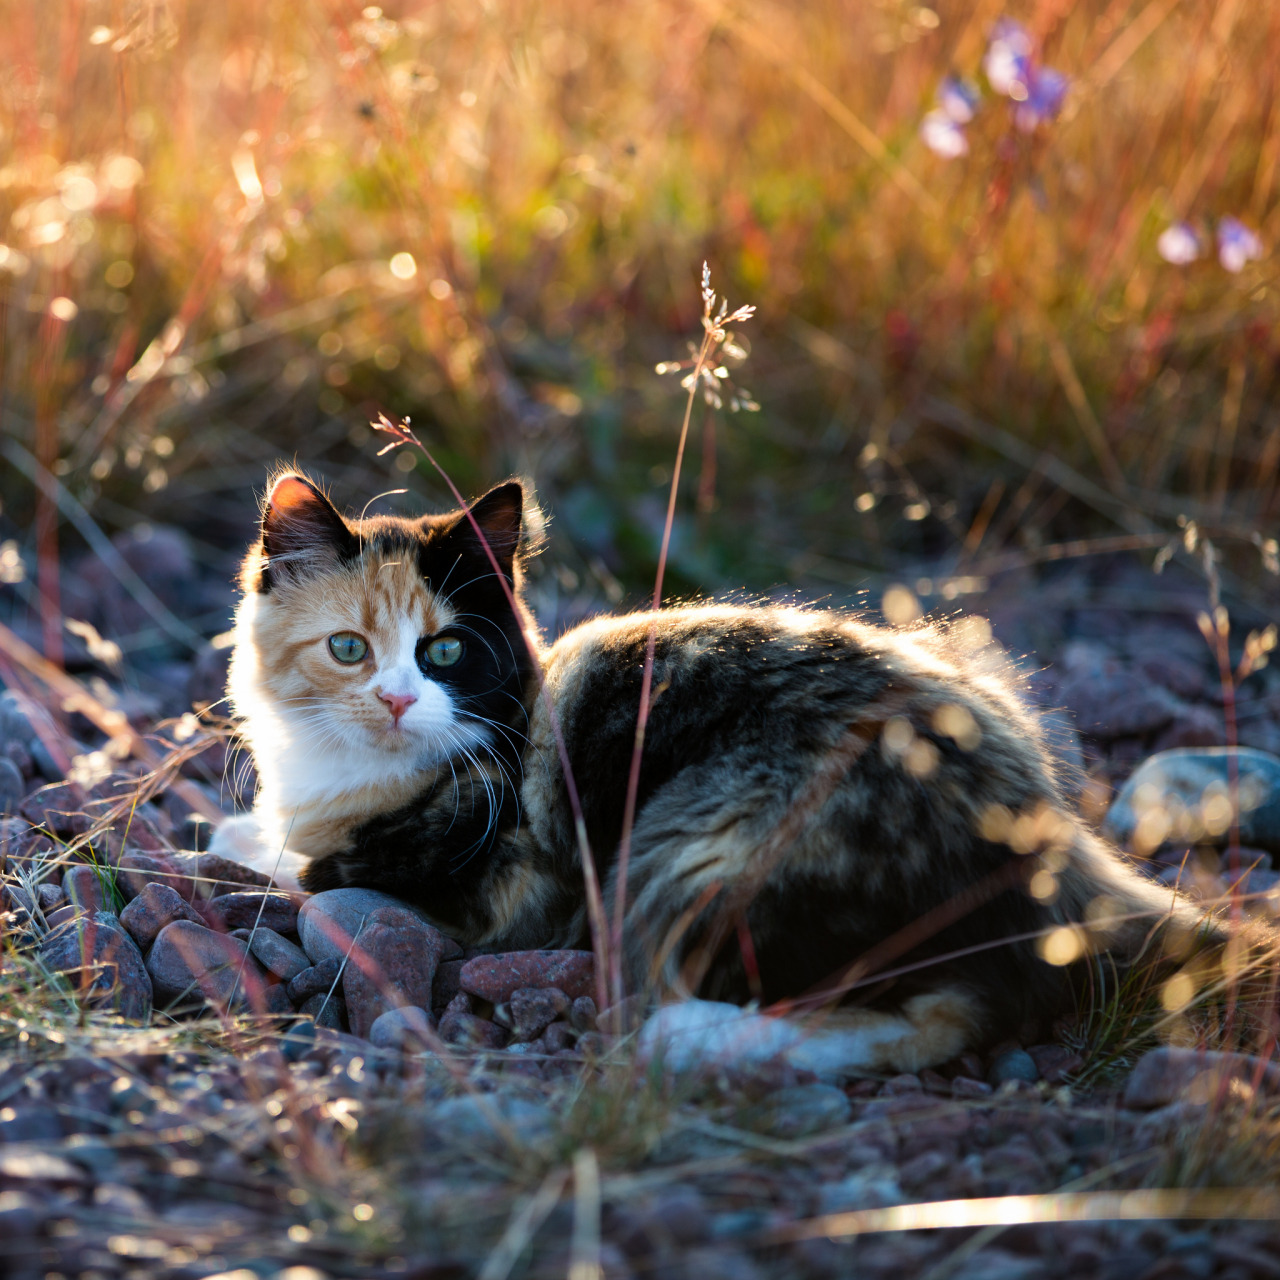
\includegraphics{Pictures/FrontCover.jpg}}} % Image background
\centering
\vspace*{11.3cm}
\par\normalfont\fontsize{35}{35}\sffamily\selectfont

\begin{center}
    % List of Latex Colour names here: https://www.overleaf.com/learn/latex/Using_colours_in_LaTeX
    \textbf{\color{Apricot} \mytitle}  % Modify the name of the colour used to suit your image
    
    \textbf{\color{White}(\ILMCode)} % Modify the name of the colour used to suit your image
    
    \color{white}Uniandes\par % Modify the name of the colour used to suit your image
    
    \vspace*{0.5cm}
    \color{Apricot}\author % Modify the name of the colour used to suit your image
    
    (\id)\par  
\end{center}

\endgroup

%----------------------------------------------------------------------------------------
%	COPYRIGHT PAGE
%----------------------------------------------------------------------------------------


\newpage
~\vfill
\thispagestyle{empty}

\noindent \textbf{Vectorial Calculus - }
\vspace{0.5cm}

\noindent 
\vspace{1cm}

\noindent \textit{First release, \date} % Printing/edition date

%----------------------------------------------------------------------------------------
%	TABLE OF CONTENTS
%----------------------------------------------------------------------------------------

\chapterimage{Heading1.jpg} % Table of contents heading image

\pagestyle{empty} % No headers

\tableofcontents % Print the table of contents itself

%\listoftables %uncomment this if you want to print the list of tables at the start

\pagestyle{fancy} % Print headers again


%----------------------------------------------------------------------------------------
%	Glossary
%----------------------------------------------------------------------------------------

\chapterimage{Heading1.jpg} % Table of contents heading image

\printglossaries



%----------------------------------------------------------------------------------------
%	First set of related questions
%----------------------------------------------------------------------------------------

\chapterimage{Heading2.jpg}
\chapter{Introduction}

\begin{flushright}
    \textit{Go big or go home.}
\end{flushright}

Vectorial calculus is what the title says pretty much, the act of using methods
proper to calculus on vectorial spaces, for the topic of this class generally referring to
merely 3-dimensional ones, at the end of this book you should be able to:

\begin{itemize}
    \item 
\end{itemize}

\vspace{20px}
\vspace{0.5cm} % Adds some vertical whitespace, easier to read

%--------------------------------------------------------------
%	More sections?
%----------------------------------------------------------------------------

\chapter{Linear Algebra Concepts}
\section{Vectors on a three-dimensional space.}

given an $ \mathbb{R}^3 $ space and a point in that space $ P = (a,b,c) $,
we can describe a vector by either connecting the point $ P $ to another point $ Q $, or
by assuming the origin of this space (point $ (0,0,0) $), this is a mathematical object with both a
direction and a magnitude. The direction is given by an angle and the 
magnitude is given by $\sqrt{a_1^2 + a_2^2 + a_3^2}$

As an example, let's assume the vector given by $ P = (1,2,1) $:
\begin{center}
    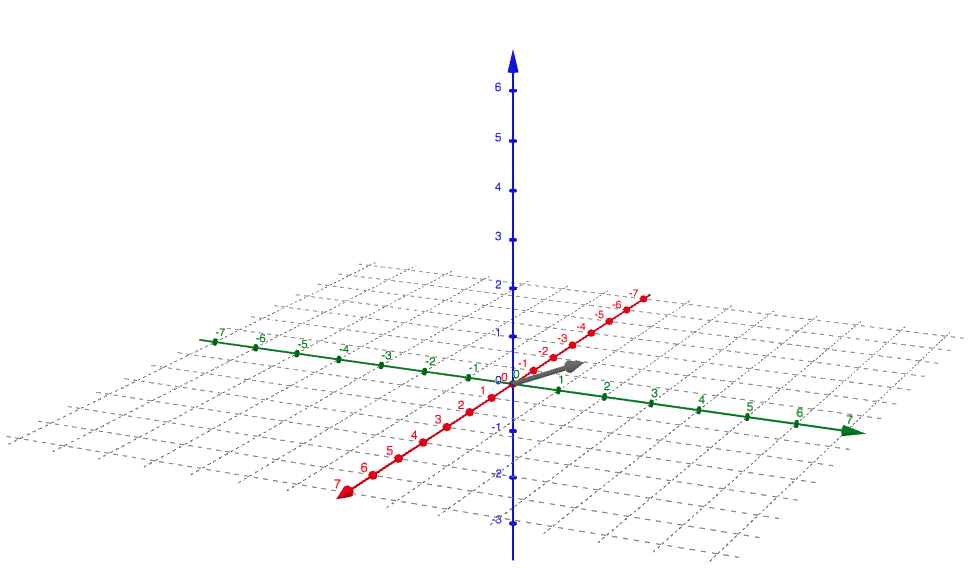
\includegraphics[scale=0.35]{vector_1.png}

    \textit{Vector formed by $ P = (1,2,1) $}
\end{center}

For this vector, we can calculate the magnitude by replacing the vectorial components by 
the magnitudes of the individual directions, resulting in:

%\begin{gather}
 %    \sqrt{1^2 + 2^2 + 1^2} \\
%
 %    \sqrt{1+4+1} \\
  %  
   %  \sqrt{6} \\
%\end{gather}

\textit{Note, in this course we will be mostly only concerned with }$ \mathbb{R}^3 $
\subsection{Addition and Subtraction}

We can take any $ \vec{a} $ and $ \vec{b} $ vectors on the same space and add them to each other
in the form:

\begin{equation}
    \begin{bmatrix}
        a_1 \\
        a_2 \\
        a_3 \\
    \end{bmatrix}
    +
    \begin{bmatrix}
        b_1 \\
        b_2 \\
        b_3 \\
    \end{bmatrix}
    = 
    \begin{pmatrix}
        a_1 + b_1\\
        a_2 + b_2\\
        a_3 + b_3\\
    \end{pmatrix}
\end{equation}

Such form remains in the case we can do subtraction, which is expressed on the equation:

\begin{equation}
    \begin{bmatrix}
        a_1 \\
        a_2 \\
        a_3 \\
    \end{bmatrix}
    -
    \begin{bmatrix}
        b_1 \\
        b_2 \\
        b_3 \\
    \end{bmatrix}
    = 
    \begin{pmatrix}
        a_1 - b_1\\
        a_2 - b_2\\
        a_3 - b_3\\
    \end{pmatrix}
\end{equation}

This kind of operations have certain properties, shown as:
\begin{gather}
    (\alpha + \beta)\vec[v] = \alpha\vec{v} + \beta\vec{v} \\
    \vec{v} * 1 = \vec{v} \\
    \vec{v} * \vec{0} = \vec{0} \\
    \beta \vec{v} = 
    \begin{pmatrix}
        \beta a_1\\
        \beta a_2\\
        \beta a_3\\
    \end{pmatrix}
\end{gather}

Two vectors $ \vec{a} $ and $ \vec{b} $ are equal if and only if:
\begin{equation}
    \begin{cases}
        \vec{a} \exists \mathbb{R}^3 \\
        \vec{b} \exists \mathbb{R}^3
    \end{cases}
    \implies
    \begin{pmatrix}
        a_1 = b_1\\
        a_2 = b_2\\
        a_3 = b_3\\
    \end{pmatrix}
    \text{
        \textit{note: this can be generalized to 'n' dimensions larger than 0}}
\end{equation}

in either case,  $ \vec{0} $ is the identity of the operation, therefore:
\begin{equation}
    \vec{a} + \vec{0} = \vec{a}
\end{equation}


\subsection{Bases}

A base in $ R^n $ can be found though $ n $ vectors on that plane, such as it 
would happen in $ R^2 $ with:

\begin{equation}
    \lambda \vec{u} + \mu \vec{v}| \lambda , \mu \exists \mathbb{R}
\end{equation}

this equation will form a parallelogram that can express the distorsion of space when
compared to a reference system, which generally is the canonical base formed by the identity.

\subsection{Dot product}
Assume two equal-length vectors of the sort:
\begin{equation}
    \begin{cases}
       \vec{a} = (a_i * n | n \exists \mathbb{R}); |\vec{a}| \exists \mathbb{R}  \\
       \vec{b} = (b_i * n | n \exists \mathbb{R}); |\vec{b}| \exists \mathbb{R} 
    \end{cases}
\end{equation}

in case we wanted to do obtain a scalar number, that corresponded to the sum of the internal products
we could obtain:

\begin{equation}
    A \centerdot B = ||\vec{A}|| ||\vec{B}||  \cos \theta
\end{equation}

for cartesian vectors, we can write this as:
\begin{gather}
    \vec{a} \centerdot \vec{b} = 
    \begin{pmatrix}
        a_1 \\
        a_2 \\
        a_3
    \end{pmatrix}
    \centerdot
    \begin{pmatrix}
        b_1 \\
        b_2 \\
        b_3
    \end{pmatrix}
    = a_1 b_1 + a_2 b_2 + a_3 b_3 \exists \mathbb{R}
\end{gather}


where $ \theta $ is the angle between both vectors. We can get it by calculating

$$ \cos \theta = \frac{\vec{u} x \vec{v}}{||\vec{u}||*||\vec{u}||} $$

If perpendicular, we can assume:

$$ \vec{u} \centerdot \vec{v} = 0 $$

\subsubsection{Notable cases.}

With these rules, we can infere a few interesting cases, which we'll be able to interpolate stuff with.

\paragraph*{Implications}

\begin{itemize}
    \item $ \theta < \frac{\pi}{2} \implies \cos \theta > 0 $
    \item $ \theta > \frac{\pi}{2} \implies \cos \theta < 0 $
    \item $ \theta = \frac{\pi}{2} \implies \cos \theta = 0$
\end{itemize}

\paragraph{Addendum: cosine values}

In vectorial calculus, we'll have certain notable angles that will appear often in exercises.
we can use fractions to get them approximated to numerical values, such values are listed on this table:

\begin{center}
    \begin{tabular}{||c c c||} 
     \hline
     $ \cos 0^o $ & $ \frac{4}{\sqrt{2}} $ & 1\\ [0.5ex] 
     \hline
     $ \cos 30^o $ & $ \frac{3}{\sqrt{2}} $ & ?\\ [0.5ex] 
     \hline
     $ \cos 45^o $ & $ \frac{2}{\sqrt{2}} $ & ?\\ [0.5ex] 
     \hline
     $ \cos 60^o $ & $ \frac{1}{\sqrt{2}} $ & $ \frac{1}{2} $\\ [0.5ex] 
     \hline
     $ \cos 90^o $ & $ \frac{0}{\sqrt{2}} $ & 0\\ [0.5ex] 
     \hline
    
    \end{tabular}
    \end{center}

\paragraph*{Addendum 2: Triangular inequality}

The triangular inequality affirms that:

$ ||\vec{u}+\vec{v}|| \le ||\vec{u}||+||\vec{v}|| $

\subsection{Cross product}

A cross product is, much like the dot product, an operation that seeks to multiply the values between
two vectors. it can be annotated as:

\begin{gather}
    \vec{u} \text{x} \vec{v} = 
    \begin{pmatrix}
        u_1 \\
        u_2 \\
        u_3 \\
    \end{pmatrix}
    *
    \begin{pmatrix}
        v_1\\
        v_2\\
        v_3\\ 
    \end{pmatrix}
    =
    \begin{pmatrix}
        u_2 v_3 - u_3 v_2\\
        u_3 v_1 - v_1 u_3\\
        u_1 v_2 - u_2 v_1 \\ 
    \end{pmatrix}
\end{gather}

This is a non-commutative operation, changing the order of signs will cause the signs to invert,
seen mathematically as:

$$ \vec{u} x \vec{v} = -(\vec{v} x \vec{u}) $$

The vector that the cross product produces is perpendicular to both evaluated vectors.


we can also use the norm of this cross product as a way to calculate the area of the paralleleipied form 
triangulated by $\vec{u}$ and $\vec{v}$ as $$ A = ||\vec{u}x \vec{v}|| $$ 
This can also work for three-dimensional paralleleipied in the following formula:

\begin{equation}
    |\vec{w} \centerdot (\vec{u}x\vec{v})| = ||\vec{w}|| * ||\vec{u}x\vec{v}|| * |\cos \vartheta| 
\end{equation}

we can also say, from this:


\begin{equation}
    \vec{w} \centerdot (\vec{u}x\vec{v}) = \vec{u} \centerdot (\vec{v}x\vec{w}) = \vec{v} \centerdot (\vec{w}x\vec{u})
\end{equation}

\subsection{Determinants}

a determinant is defined as:

\begin{equation}
    det
    \begin{pmatrix}
        a & b \\
        c & d \\
    \end{pmatrix}
\end{equation}

\section{Describing objects in a space.}

\subsection{Lines}

A line is a geometrical object of the form:

\begin{equation}
    r(t) = t \vec{v} + P, t \exists \mathbb{R}
\end{equation}

generating it requires a point and a vector. Point defined by P, and vector defined by an offset 't' and a vector '$\vec{v}$'

\textbf{Example}
\textit{Find the equation of a line 'l' that crosses $A=(2,1,1)$ and $B=(3,5,7)$}

for this, we'll establish the following formula:
\begin{gather}
    l(t) =
    \begin{pmatrix}
        A_1\\
        A_2\\
        A_3\\
    \end{pmatrix}
    +
    t 
    \begin{pmatrix}
        B_1-A_1\\
        B_2-A_2\\
        B_3-A_3\\
    \end{pmatrix}
\end{gather}

Instanced, for this specific case, as:
\begin{gather}
    l(t) =
    \begin{pmatrix}
        2\\
        1\\
        1\\
    \end{pmatrix}
    +
    t 
    \begin{pmatrix}
        3-2\\
        5-1\\
        7-1\\
    \end{pmatrix}
    \\
    l(t) =
    \begin{pmatrix}
        2\\
        1\\
        1\\
    \end{pmatrix}
    +
    t 
    \begin{pmatrix}
        1\\
        4\\
        6\\
    \end{pmatrix}
\end{gather}

Answer is equation 2.15, this can be later expanded into a parametric or simetric form of this line. But before we do that, let's try expanding the reason this works:

\textbf{Example 2}
\textit{Find the equation of the line that joins points $P=(1,2,1)$ and
$ Q=(-1,3,4) $}

we can find the line that joins two points by subtracting the vectors that join them, let's take a look at the 
cartesian plane where we indicate 'P' and 'Q':

\subsection{Vector Projection}

A vector can be projected through the equation:

\begin{equation}
    \frac{\vec{u} \centerdot \vec{v}}{||\vec{v}||^2} \vec{v}
\end{equation}

\subsection{Euclidian Planes}

A plane is the union of all points in a 2-dimensional subset of $ \mathbb{R^3} $ defined by a formula of the type:
\begin{equation}
    i_1 A + i_2 B + i_3 C = D = (D \centerdot || \vec{n} ||)
\end{equation}

Where $ \vec{n} $ is also written as:
\begin{equation}
    \vec{n} = \begin{pmatrix}
        a \\
        b \\
        c
    \end{pmatrix}
\end{equation}

It can be determined by 
\begin{itemize}
    \item three points in $ \mathbb{R^3} $
    \item Two vectors and a point in $ \mathbb{R^3} $
    \item a point and the normal vector in $ \mathbb{R^3} $
\end{itemize}

\section{Cylindrical and spherical coordinates.}

When trying to define parts of a line in algebra, we'll usually be looking at
coordinates, be them polar or cartesian. In either case, their information can be 
converted to the other system through the following formulas.

\begin{gather}
    \begin{cases}
        \rho = \sqrt{x^2+y^2} \\
        \theta = \arctan(\frac{y}{x})
    \end{cases}
    \text{\textit{cartesian to polar}}\\
    \begin{cases}
        \alpha_x = \rho \cos \theta \\
        \alpha_y = \rho \sin \theta
    \end{cases}
    \text{\textit{polar to cartesian}}
\end{gather}

Cartesian coordinates generally translate well to other dimensional spaces, such as would be the case
for $ \mathbb{R}^3 $, however, polar coordinates as we know them usually aren't as translatable in a direct
manner, and expressing them in three-dimensional spaces might be better suited to 
be expressed on a cylindrical or spherical condition. 
\subsection{Cylindrical coordinates}
In the case of cylindrical coordinates, the translation is probably the most intuitive, by computing
a cylinder with polar coordinates that indicate an (x,y) position, and a 'Z' variable indicating height 
that allows us to project the vector on a third dimension, this 'z' variable is exactly the same as it would be
on a cartesian model. We can express it like such:

$ \vec{v} = ( \rho, \theta, Z) $

conversion to a cartesian model can be expressed as:

\begin{gather}
    \vec(\alpha) =
    \begin{cases}
        \alpha_x = \rho \cos \theta \\
        \alpha_y = \rho \sin \theta \\
        \alpha_z = Z
    \end{cases}
    \text{\textit{Cylindrical to cartesian}}
    \\
    \vec(\alpha) =
    \begin{cases}
        \rho = \sqrt{x^2 + y^2} \\
        \theta =  \arctan(\frac{y}{x}) \\
        Z = Z
    \end{cases}
    \text{\textit{Cartesian to Cylindrical}}
\end{gather}

\subsection{Spherical coordinates}

A spherical coordinate is formed by a tuple:

\begin{gather}
    (\rho, \theta ,\phi);
    \begin{cases}
        \rho \geq  0 \\
        0 \le \theta \le 2\pi \\
        0 \le \phi \le \pi    
    \end{cases}
\end{gather}

Where $ \rho $ is the magnitude of the vector, $\theta$ is the (x,y) coordinates, and
$\phi$ is the (y,z) angle. They must adhere to the following for it to be geometrically coherent:

\begin{equation}
    \begin{cases}
        \rho > 0 \\
        0 \le \phi \le \pi \\
        0 \le \theta \le 2\pi
    \end{cases}
\end{equation}

this tuple can generate two vectors:
\begin{equation}
    \begin{cases}
        \rho \sin \phi\\
        \rho
    \end{cases}
\end{equation}

And can be converted to a cartesian model as such:

\begin{gather}
    \vec(\alpha) =
    \begin{cases}
        \alpha_x = \rho \sin \phi \cos \theta \\
        \alpha_y = \rho \sin \phi \sin \theta \\
        \alpha_z = \rho \cos \phi
    \end{cases}
    \text{\textit{Spherical to cartesian}} \\ 
    \vec(\alpha) =
    \begin{cases}
        \rho = \sqrt{x^2 + y^2 + z^2} \\
        \theta =  \arctan(\frac{y}{x}) \\
        \phi = \arccos(\frac{z}{\rho})
    \end{cases}
    \text{\textit{Cartesian to Spherical}}
\end{gather}

\paragraph{Example}
Imagine the following spherical vector:
$$
\begin{cases}
    \rho = 2 \\
    \theta = \frac{\pi}{2}\\
    \phi = \frac{\pi}{4}
\end{cases}
$$

\textit{How do we convert it to a cartesian vector?}

We'll get the vector by simply replacing the previous formulas with the 
values provided as it follows:

\begin{equation}
    x = 2 \sin(\frac{\pi}{4}) \cos(\frac{\pi}{2}) \\
    y = 2 \sin(\frac{\pi}{4}) \sin(\frac{\pi}{2}) \\
    z = 2 \cos(\frac{\pi}{4})
\end{equation}

We can also invert this equation and get a cartesian vector to its spherical form
through the following formula:
\begin{gather}
    \begin{cases}
        \rho = \sqrt{x^2 + y^2 + z^2} \\
        \theta = \arctan{\frac{y}{x}} \\
        \phi = \arccos{\frac{z}{\sqrt{x^2 + y^2 + z^2}}}
    \end{cases}
    \text{\textit{Cartesian to Spherical}}
\end{gather}

Such a model works, as we might imagine, like a sphere. where we express the possible vectors
through a sphere of $ \rho $ radius.

\section{n-dimensional Euclidian Spaces}

in an n-dimensional euclidian space, we can determine:

\begin{equation}
    \mathbb{R}^n, \vec{x} \begin{pmatrix}
        x_1
        \dots
        x_n
    \end{pmatrix}
    ; \mathbb{C}
    \text{\textit{ Operations:}}
    \begin{cases}
        \vec{x}+\vec{y} \\
        \alpha \vec{x} \\
        \vec{x} \centerdot \vec{y} \\
    \end{cases}
\end{equation}


\subsection{Cauchy-Schwartz Inequality}

This inequality determines that the internal product is lesser or equal to the
multiplication of the norms of two vectors, written as:

\begin{gather}
    \text{Let: } \vec{x},\vec{y} \exists \mathbb{R}^n \text{ then: }\\
    |\vec{x}\centerdot\vec{y}| \le ||\vec{x}|| \centerdot ||\vec{y}||
\end{gather}

and it is equal if and only if:

\begin{equation}
    \vec{x} = \lambda \vec{y} \text{ or either } \begin{cases}
        \vec{x} = 0 \\
        \vec{y} = 0
    \end{cases}
\end{equation}

\section{Matrices}

A matrix is a numerical representation of values in $ \mathbb{R}^n $. They can represent 
planes, vectors, or even hyperplanes in $ \mathbb{R}^n | n > 3 $. An example in $\mathbb{R}^2$
would be:

\begin{equation}
    \begin{pmatrix}
        a & b \\
        c & d
    \end{pmatrix}
\end{equation}

Notable matrices include:
\begin{itemize}
    \item Identity: $ \begin{pmatrix}
        1 & \dots & 0 & \dots & 0 \\
        0 & \dots & 1 & \dots & 0 \\
        0 & \dots & 0 & \dots & 1
    \end{pmatrix} $ = Id
\end{itemize}

\subsection{Inverible Matrices}

We can invert a matrix if a $ B_{nxn} $ matrix exists such as:
\begin{equation}
    AB = BA = Id
\end{equation}

we can also use the determinant to check this, as:

\begin{equation}
    det(A) \begin{cases}
        = 0 \text{: is Invertible} \\
        \neq 0 \text{: is not Invertible} \\
    \end{cases}
\end{equation}

\subsection{Matrix multiplication}

We can multiplicate a matrix by another one if we define the multiplication as:

\begin{equation}
    AxB = C_{ij} = \sum_{k = 1}^{n} a_{ik} b_{jk}  
\end{equation}

\paragraph{Example}

We want to multiply two matrices as:

\begin{equation}
    \begin{pmatrix}
        a & b\\
        c & d
    \end{pmatrix}
    x
    \begin{pmatrix}
        1 & 2 \\
        0 & 1
    \end{pmatrix}
\end{equation}

Therefore if we try doing AxB and BxA:

\begin{gather}
    AxB =
    \begin{pmatrix}
        a & 2a + b \\
        c & 2c + d
    \end{pmatrix}\\
    BxA =
    \begin{pmatrix}
        a+2c & b + 2d \\
        c & d
    \end{pmatrix}\\
\end{gather}

As we can see, matrix multiplication is not commutative, but rather it is defined
by the order on which A and B are written


$$ Ae_j = A_j $$

\chapter{Functions and Equations}

In mathematics, even though similar, functions and equations 

\section{Geometry of functions with values in $ \mathbb{R} $}

We can affirm that a function is two or three dimensional if, respectively:

\begin{gather}
    y = f(x) \implies \begin{cases}
        (x,y): y = f(x), x \exists D(f)
    \end{cases} \\
    z = f(x,y) \implies \begin{cases} 
    (x,y,z): z = f(x,y), (x,y) \exists D(f)
    \end{cases}
\end{gather}

\pagebreak
\paragraph*{Example:}
\textit{3,1,1: Graphicate the following:}
$$ z = \frac{6-x-2y}{3} $$
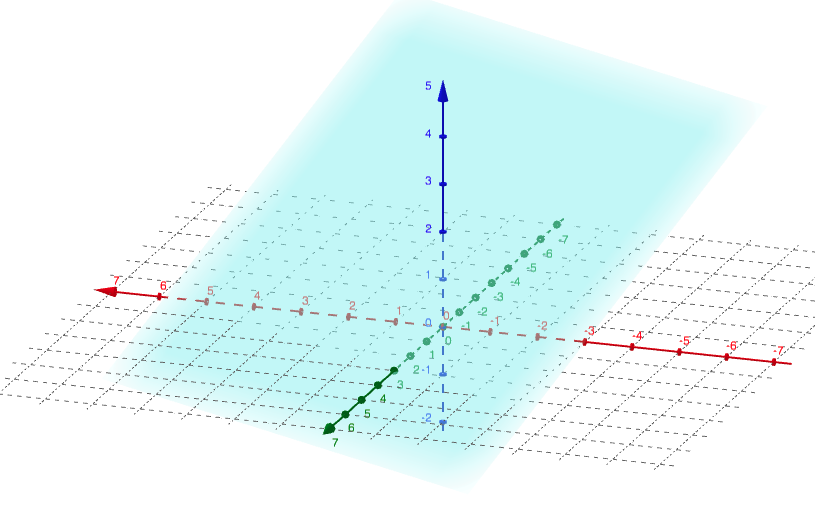
\includegraphics[scale = 0.5]{Pictures/plane3,1.png}

As we can see, the graph makes sense because:

\pagebreak
\textit{3,1,2: Graphicate the following:}

$$ z = 1-x = f(x,y) $$
\includegraphics*[scale=0.5]{plane3,1,2.png}
\pagebreak

\textit{3,1,3: Graphicate the following:}

$$ z = x^2 + y^2 $$

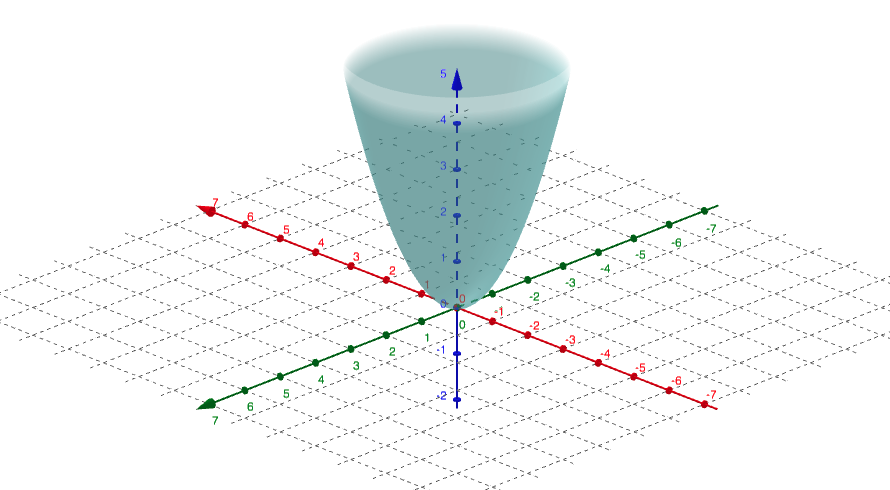
\includegraphics[scale = 0.5]{Pictures/plane3,1,3.png}
this is a three-dimensional parabola, also called more correctly as a circular paraboloid, comparable to it's two dimensional form, yet 
working on another dimension.

it can guarantee:

$$ \begin{cases}
    x = 0: z = y^2 \\
    y = 0: z = x^2
\end{cases}$$

and this equation can be deduced through this behavior. As:

$$ z = z_0 : x^2 + y^2 = z $$

there are level curves, which project the curve generated by such mathematical artifacts as a two dimensional
spherical object. Fields like topology or other 3-dimensional inclined math might regularly use it
when measuring space. In any case, a level curve could be illustrated as such:
\begin{center}
    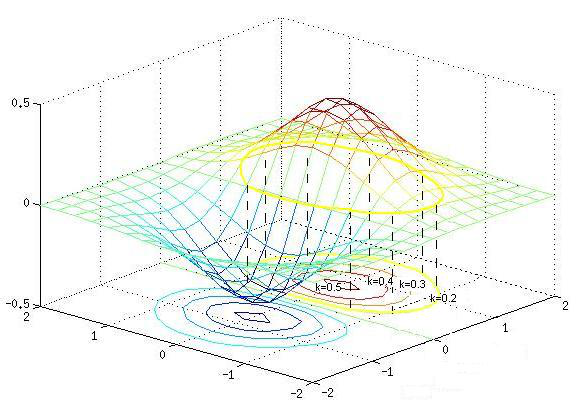
\includegraphics[]{Pictures/GraphCurves.png}    
    \textit{taken from: www.math.tamu.edu}
\end{center}

\section{Equations}

An equation, although similar to a function such as the ones studied so far,
can be distinguished by some particularities they present: 

$$ x^2 + y^2 + z^2 = 1$$

A few examples of objects described by equations are:

\subsection{Planes}

A plane is a 2-dimensional shape that can be expressed as:
\begin{equation}
    Ax + By + Cz = Ax_0 + By_0 + Cz_0
\end{equation}

There are different ways of getting the values regarded in this shape, as seen in 2.2.3 of these class notes, and we will mostly
do it by passing different geometrical expressions to a point and a vector normal to the plane, and replacing the vector 
on A,B,C, and the point in $ x_0, y_0, z_0 $

\paragraph{Example}

Find a plane normal to: $ \vec{n} = \begin{pmatrix}
    1 \\
    2 \\
    3 \\
\end{pmatrix} $
That passes through:
$ P = \begin{pmatrix}
    1 \\
    1 \\
    1 \\
\end{pmatrix} $

We replace fot this as following:

\begin{equation}
    1x + 2y + 3z = 1*1+2*1+3*1 \implies 1x + 2y + 3z = 6
\end{equation}


\subsection{Elipsoids}

An elipsoid is defined by the following equation:
\begin{equation}
    (\frac{x}{a})^2+(\frac{y}{b})^2+(\frac{z}{c})^2 = 1
\end{equation}


\subsection{Hyperboloid}

a Hyperboloid can be seen as:
\begin{equation}
    (\frac{x}{a})^2+(\frac{y}{b})^2 = (\frac{z}{c})^2 + 1
\end{equation}

\subsection{Cilinders}

The general formula of a cylinder is:

\begin{equation}
    (\frac{x}{a})^2+(\frac{y}{b})^2 = 1
\end{equation}

The level curves of this shape will never change when projected on a plane.

\subsection{Parabolic}

The general formula of a parabolic is:

\begin{equation}
    y = ax^2
\end{equation}

\subsection{Spheres}

\begin{equation}
    \begin{cases}
        x^2+y^2+z^2 = r^2 \\
        z \geq 0
    \end{cases}
\end{equation}

\subsection{Paraboloid}

The general formula of a paraboloid is:

\begin{equation}
    z = (\frac{x}{a})^2 + (\frac{y}{b})^2
\end{equation}

This shape has a variation, called a hyperbolic paraboloid:


\begin{equation}
    z = (\frac{x}{a})^2 - (\frac{y}{b})^2
\end{equation}

It will look like this when graphicated:
\begin{center}
    \includegraphics*[]{Pictures/hyperbolic_paraboloid.png}    
\end{center}

\chapter{Limits and continuity}
\subsection*{Sets and disks}
An open disk of radio 'r' and contourn $\vec{x}$ can be defined as


\begin{equation}
    \text{Let: }\vec{x}\exists\mathbb{R}^n , r > 0 \\ D_r = \{ \vec{x} \exists \mathbb{R}^n: ||\vec{x} - \vec{x_0} || < r \}
\end{equation}

and a disk that includes the internal values could be defined as 

\begin{equation}
    \text{Let: }\vec{x}\exists\mathbb{R}^n , r > 0 \\ D_r = \{ \vec{x} \exists \mathbb{R}^n: ||\vec{x} - \vec{x_0} || \le r \}
\end{equation}

Both of these are an important definition of what we'll call a \textbf{set}. 

let $$ \mu \subseteq \mathbb{R}^n $$ we can say that $\mu$ is an open set if  for any point $x_0 \exists \mu$
there exists a r>0 such as $$D_r(x_0) \subseteq \mu$$

Such sets have a mathematical structure called frontier points that can be defined as:
\paragraph*{Frontier point}
Let $ A \subseteq \mathbb{R}^n $; a point '$x \exists \mathbb{R}^n$' is a frontier point if any $ \vec{x} $
vecinity contains a point of A and at least a point outside of A

\paragraph*{Example}

Prove that '$A = (x,y)\exists\mathbb{R}^2: y > 0$' is an open set

Given that the open set can be inferred by a disk, we can affirm:

\begin{gather}
    \implies y>0 \implies r = \frac{y}{2} > 0 \\
    \text{If : }(a,b)\exists D_r(x,y)\\
    | b-y | \le \sqrt{(a-x)^2 + (b-y)^2} < r = \frac{y}{2} \\
    |b-y| < \frac{y}{2}\\
\end{gather}

\section{Limits}
A limit can be defined as

$ \lim_{x \to a} f(x) = L $

Where:

$ \forall \epsilon > 0 \exists \varrho > 0: | f(x) - L | < \epsilon $
for all X, such as 

$ 0 < |x-a| < \vartheta $

Or when said in words; "for every epsilon greater than zero that exists in a theta greater than zero, the function of value x minus L is lesser than epsilon for all X, such as the norm is greater than zero and smaller than theta".

For a limit to exist, we need three conditions to be met:

\begin{itemize}
    \item there is a left limit
    \item there is a right limit
    \item they're equal
\end{itemize}


\subsubsection{Multivariable limits}

a limit in a multi variable plane can be defined as: 

\begin{gather}
    \lim_{(x,y) \to (a,b)} = \vec{L}
\end{gather}

Meaning that we can force $ |f(x,y)-L|$ to be as near to zero as posible, making
(x,y) and (a,b) as close as possible without them actually ever touching each other.

Or, more formally;

\begin{gather}
    f: \mathbb{R}^n \to \mathbb{R}^m \\
    \text{Let: } f: A \subseteq \mathbb{R}^n \rightarrow \mathbb{R}^n \text{and :}\\
    \text{let $ \vec{x_0} \exists A $ or $ \vec{x_0} \exists \varTheta A $ }\\
    \lim_{x \to x_0} f(\vec{x}) = L \exists \vartheta \exists A \implies 0 < ||\vec{x} - \vec{x_0}|| < \vartheta, \implies ||f(\vec{x})-L||<\epsilon
\end{gather}

\subsection{Differentiation}

a function in a single variable can have every single point on a curve being approximated to
a line, called a tangent. This z = (x,y) line variable can be defined by partial derivatives, that
can be described as:
\begin{equation}
    z_x = \frac{D_z}{D_x} = \frac{D_f}{D_x} (x,y) = \lim_{h \to 0} = \frac{(x+h,y)-f(x,y)}{h} 
\end{equation}
\begin{equation}
    \frac{d_f}{d_y}(x,y) = \lim_{h \to 0} = \frac{(x,y+h)-f(x,y)}{h}
\end{equation}
Where 'h' is a real number that tends towards zero.

\paragraph*{Example: }
\textit{let: }
\begin{gather}
    f(x,y) = x^2-y^3 - 3x^4y
\end{gather}
\textit{then, differentiate the equation.}

\textbf{solution:}

\begin{gather}
    \frac{d_f}{d_x} = 2xy^3 - 12x^3y \\
    \frac{d_f}{d_y} = 3x^2y^2 - 3x^4
\end{gather}

When differentiating an equation on a specific variable, we take the other variables as constants.
In this example, we leave 'x' untouched when differentiating on 'y' and viceversa.

\subsection{Implicit differentiation}

We can think of an implicit derivative as the process of using partial derivatives to 
differentiate a single, more complex equation. 

\paragraph{Examples: }

\begin{itemize}
    \item a line that goes through $ \frac{y - y_0}{x - x_0} $

\end{itemize}

For three dimensions we might imagine instead of a line being the tangent, a 
plane providing the same definition and mathematical role as it, defined as:

\begin{gather}
    z = f(x, y_0) : z - z_0 = \frac{d_f}{d_x}(x, y_0)(x-x_0) \\
    z = f(x_0, y) : z - z_0 = \frac{d_f}{d_x}(x_0, y)(y-y_0)
\end{gather}

and with both this derivatives, we can define a plane as 

\begin{equation}
    z - z_0 = a(x-x_0) + b (y-y_0) \text{\textit{Where: }} \begin{cases}
        a = \frac{d_f}{d_y}f(x_0, y_0)\\
        b = \frac{d_f}{d_x}f(x_0,y_0)
    \end{cases}
\end{equation}

IF: $ x = x_0 = 0 $ and $ y = y_0$

We can approximate a three-dimensional differentiation as 

\begin{gather}
    d_z = fx(x_0, y_0)(x - x_0) + f_yfx(x_0, y_0)(y - y_0)\\
    f(x,y) \approx f(x_0, y_0) + d_z
\end{gather}

\textit{note: tangent planes are a very popular test/quiz problem, you should
learn how to find them for such ventures, if your professor ever mentions them
in class and ESPECIALLY if they try to solve one in front of the class.}

We can say that a function $ f: \mathbb{R}^2 \to \mathbb{R} $ is differentiable if:

\begin{equation}
    \Delta f = d_f + \epsilon_1 \Delta x +\epsilon_2 \Delta y 
\end{equation}

\noindent This deffinition is a bit hard to applicate, so we'll use the differentiation criteria for 
looking for appliability.

\textit{Appliability Criteria: }
We will say it is possible to differentiate a function if every partial derivative in $\frac{d_f}{d_{xj}}$
and if they're continuous in an open set 'D'.

\paragraph*{Example:}
\begin{gather}
    f(x,y) = \begin{cases}
        0 \implies (x, y) = (0,0) \\
        x^2 + y^2 \implies (x,y) \neq (0,0)
    \end{cases} \\
    \frac{df}{dx} (0,0)= \lim_{h \to 0}  \frac{f(h, 0) - f(0,0)}{h} = \lim_{h \to 0}  \frac{0 - 0}{h} = 0 \\
    \text{BUT THEN, that means a partial derivative for (0,0) does not exist,}\\ \text{ therefore this is not a continuous function.} \\
    \lim_{(x,y) \to (0,0)}  \frac{xy}{x^2+y^2} NE
\end{gather}

\subsection{Examples}
\begin{itemize}
    \item Solve:

\begin{equation}
    \lim_{(x,y) \to (0,0)}  \frac{\cos - 1 - \frac{x^2}{2}}{x^4+y^4}
\end{equation}

This limit \textbf{DOES NOT EXIST}:

because going by paths we can assume:

$$<x=0>$$

Would imply:
\begin{gather}
    \lim_{y \to 0} \frac{\cos 0 - 1 - \frac{0^2}{2}}{0^4 + y^4} \\
    \lim_{y \to 0} \frac{0}{y^4} = \lim_{y \to 0} 0 = 0
\end{gather}

$$<y=0>$$

Would imply:
\begin{gather}
    \lim_{x \to 0} \frac{\cos x - 1 - \frac{x^2}{2}}{x^4} \implies \frac{0}{0} \\
    \text{<l'Hopital because of indetermination>}\\
    \lim_{x \to 0} \frac{- \sin x - x}{4x^3} \\
    \text{<l'Hopital because of indetermination... again.>} \\
    \lim_{x \to 0} \frac{- \cos x - 1}{12x^2} \\
    \dots
\end{gather}

...and it will never stop differentiating until a $\mathbb{R}$ value is divided by 0, which
isn't possible without adding multiple things to our framework of reference, maybe imaginary numbers or
something.


we can graphicate such a function as:

\begin{center}
    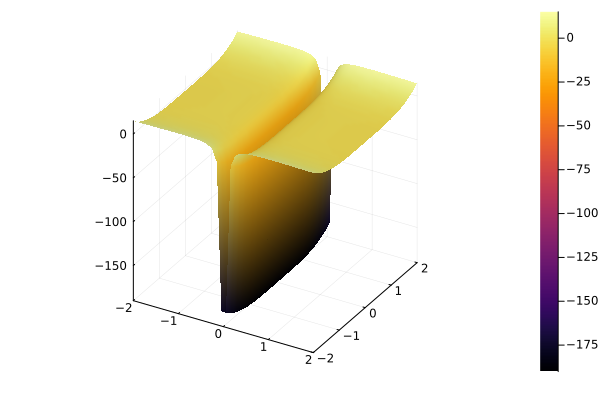
\includegraphics[scale=0.5]{Pictures/4131.png}    
\end{center}

Would imply:
\end{itemize}
\section{Continual Functions}

A function can be defined as continual if a limit can be described as:

\begin{itemize}
    \item $$\lim_{\vec{x} \to \vec{x}_0}f(x) = f(X_0) = f(\lim_{\vec{x} \to \vec{x_0}} \vec{x})$$
\end{itemize}

This would mean that a limit is replaceable by a function where the limit of $\vec{x}$ 
is described according to the mathematical rules that define a function. 
if a function is continual and has $\frac{D_{fi}}{D_{xj}}$ then it's differentiable


\section{Tangent Planes}
 We tangentially touched this topic on implicit differentiation, however, to define more 
 formally a tangent plane,
 
 Let:

 \begin{gather}
    f: A \subseteq \mathbb{R}^2 \to R \\
    \vec{\Delta} f (x,y) = < \underbrace{\frac{D_f}{D_x} (x,y)}_\text{Partial Derivative of X}, \underbrace{\frac{D_f}{D_y} (x,y)}_\text{Partial Derivative of y}> \\
    f(x_0, y_0) + D(f(\vec{x})) (\vec{x}-\vec{x_0})
 \end{gather}


\section{Derivative Properties}
\subsection{Constant multiple rule}
$$ \frac{\delta}{\delta_x}(c f(x,y)) = c \frac{\delta}{\delta_x}(f(x,y)) $$
\subsection{Sum rule}
$$\frac{\delta}{\delta_x}(f(x,y) + g(x,y)) = \frac{\delta_f}{\delta_x} f(x,y) + \frac{\delta_g}{\delta_x} g(x,y)$$
\subsection{Product rule}
$$\frac{\delta}{\delta_x}(f(x,y) \centerdot g(x,y)) = \frac{\delta_f}{\delta_x} f(x,y) g(x,y) + \frac{\delta_g}{\delta_x} g(x,y) f(x,y)$$
\subsection{Divisor rule}
$$\frac{\delta}{\delta_x}(\frac{f}{g})(x,y) = \frac{\frac{\delta_f}{\delta_x} f(x,y) g(x,y) - \frac{\delta_g}{\delta_x} g(x,y) f(x,y)}{[g(x,y)]^2}$$
\subsection{Chain Rule}

\subsubsection{One variable}
If $\vec{u}(x)$ and $\vec{x}(t)$ are differentiable, then: 

$$\frac{\delta_u}{\delta_t} = \frac{d_y}{d_x} \frac{d_x}{d_t} = u'(x|t|) + x'(t)$$

\subsubsection{Two variables}

Given  $\vec{w}(x,y)$, $\vec{u}(x,y)$ and $\vec{v}(x,y)$, then $w(u(x,y), v(x,y))$ is differentable.

so, therefore:

\begin{gather}
    y = 
    \begin{cases}
        \frac{\delta w}{\delta x} = \frac{\delta w}{\delta u} \frac{\delta u}{\delta x} + \frac{\delta w}{\delta v} \frac{\delta v}{\delta x} \\
        \frac{\delta w}{\delta y} = \frac{\delta w}{\delta u} \frac{\delta u}{\delta y} + \frac{\delta w}{\delta v} \frac{\delta v}{\delta y} 
    \end{cases}
\end{gather}


In general, we can define this rule as 
\begin{equation}
    D(f o g) = Df(g(\vec{x_0})) Dg(\vec{x_0})
\end{equation}

\section{Gradients and directional derivatives.}

assume a 3D plane as such:

\begin{center}
    \includegraphics*[scale = 0.5]{plane.png}
\end{center}

Def: a directional derivative is given by:

\begin{equation}
    D_{\vec{u}}f(x_0,y_0) = \frac{d}{dt} f(x_0 + t u_1, y_0 + t u_2) ; t = 0
\end{equation}

And we say that if a derivative exists, then $||\vec{u}|| = 1$;
f depends on x and y, and x and y both depend on t, this can be seen mathematically as:

\begin{equation}
    \frac{df}{dx} f(x_0 + t u_1, y_0 + t u_2) \underbrace{U_1}_{\frac{dx}{dt}} + \frac{df}{dy}(x_0 + t u_1, y_0 + t u_2) \underbrace{U_2}_{\frac{dy}{dt}}
\end{equation}

from this we can observe
\begin{equation}
    D_{\vec{u}}\ f(x_0, y_0) = \vec{\Delta} f(x_0, y_0) \centerdot \vec{u} = ||\vec{\Delta} f(x_0,y_0)|| \centerdot ||\vec{u}|| \centerdot \cos \theta\\
\end{equation}

So, given this set of conditions:

\begin{gather}
    \begin{cases}
        D_{\vec{u}} f(x_0, y_0) \text{  is maximal if $ \theta $ is 0} \\
        D_{\vec{u}} f(x_0, y_0) \text{  is minimal if $ \theta $ is $\pi$}
    \end{cases}
\end{gather}

We can infer then, regarding our direction:

\begin{equation}
    \vec{u} = \frac{\vec{\Delta} f(x_0, y_0)}{||\vec{\Delta}f(x_0,y_0)||}
\end{equation}

will make the function grow faster, and:

\begin{equation}
    \vec{u} = - \frac{\vec{\Delta} f(x_0, y_0)}{||\vec{\Delta}f(x_0,y_0)||}
\end{equation}

will make it decrease faster.
 

\subsection{implicit equations}

An implicit surface equation given by $F(x,y,z) = C$ we can define, as a curve:

\begin{gather}
    \vec{r}t = <x(t),y(t),z(t)> \\
    \vec{r}t' = <x'(t),y'(t),z'(t)> 
\end{gather}

And from there we can assume that this curve is a part of S if:

\begin{gather}
    F(x(t), y(y), z(t)) = C ; \forall t
\end{gather}

Given this, F depends on x,y, and z and those three variables depend on t, allowing us
to affirm:

\begin{gather}
    F_x \frac{dx}{dt} + F_y \frac{dy}{dt} + F_z \frac{dz}{dt} \\
    \vec{\Delta} f \centerdot \vec{r}t' = 0
\end{gather}

geometrically this means the gradient is perpendicular to the tangent and therefore, the tangent plane.
to S in $(x_0,y_0,z_0)$, which can be expressed vectorially (and therefore, more usefully) as:

\begin{equation}
    \vec{\Delta}F(x_0,y_0,z_0) \centerdot \begin{pmatrix}
        x - x_0 \\ 
        y - y_0 \\ 
        z - z_0
    \end{pmatrix} = 0
\end{equation}

The line normal to S in $(x_0,y_0,z_0)$ can be defined as:

\begin{equation}
    \vec{n}(t) = \vec{x_0} + t\vec{\Delta} F(x_0,y_0,z_0)
\end{equation}

\section{Iterated Partial derivatives:}

\paragraph*{addendum}

Remember:
\begin{itemize}
    \item $f \exists C^o$ means a function is continuous
    \item $f \exists C^1$ means f' is continuous
    \item $f \exists C^k$ means the k derivative is continuous
\end{itemize}

\subsection{Iterated derivatives}
let:

\begin{equation}
    f(x,y) = x^2 y^3 - 3x^4 y
 \end{equation}

then:

\begin{gather}
    f_x(x,y) = 2xy^3 - 12x^3 y \\
    f_y(x,y) = 3x^2 y^2 - 3x^4 \\
    f_{xx} = 2y^3 - 36x^2y \\
    f_{xy} = 6xy^2 - 12x^3 \\
    f_{yx} = 6xy^2 - 12x^3 \\
    f_(yy) = 6x^2y
\end{gather}

As we can see, equations 4,51 and 4,52 are equivalent, this is because when we do
such chained differentiations, we can guarantee:

\begin{equation}
    \frac{\partial}{\partial y} (\frac{\partial f }{\partial x}) = \frac{\partial^2 f}{\partial y \partial x}
\end{equation}

\subsection{Clairaut's Theorem}

If $ f(xy), f(yx) $ are continuous, then $f_{xy} = f_{yx}$ 

\subsubsection*{Proof}

Okay, this might get a bit technical, but here we go:

As written by Kiril Datchev from Purdue\cite[]{} (give his stuff a read, it's pretty cool), we can take as a given:

By definition:
\begin{itemize}
    \item \begin{equation}
        \partial_x \partial_y f(a,b) = \lim_{h \to 0} \frac{\partial_y f(a + h, b) - \partial_y f(a,b)}{h}
    \end{equation}
\end{itemize}

So from this, we can deduce:
\begin{gather}
    \\
\end{gather}

\section{Examples}

\paragraph*{Find the gradient in P=(0,3) if $f(x,y)=2ye^{xy}+ y \cos x$} 
We can use what we know of partial derivatives to affirm:
\begin{gather}
    \vec{\Delta}f(x,y) = <2y^2 e^{xy} - y \sin x ; 2e^{xy}+2xe^{xy} + \cos x>;\\
    \text{<replace for P>};\\
    \vec{\Delta}f(0,3) = <2*3^2 e^{0*3} - 3 \sin 0 \ ; \ 2e^{0*3} + 2* 0 *e^{0*3} + \cos (0)>;\\
    \vec{\Delta}f(0,3) = <18,3>
\end{gather}

\paragraph*{Find the derivative in $f(x,y) = \frac{x}{y}$ in the point
(6,-2) and the direction of $\vec{v} = <1,3>$} 

This can be said as:
\begin{gather}
    \vec{\Delta}(x,y) = <\frac{1}{y},-\frac{x}{y^2}>;\\
    \vec{\Delta}(6,-2) = <- \frac{1}{2},-\frac{3}{2}>
\end{gather}

Given this initial state, we can then use the following declarations on this problem:

\begin{gather}
    ||\vec{v}|| = \sqrt{10};\\
    \vec{u} = \frac{\vec{v}}{||\vec{v}||} = \frac{1}{||\vec{v}||} \vec{v}
\end{gather}

And therefore, conclude:

\begin{equation}
    D_{\vec{u}}f(6,-2) = \frac{1}{\sqrt{10}} (\frac{1}{2} - \frac{9}{2}) = \frac{4}{\sqrt{10}} = -\sqrt{\frac{8}{5}}
\end{equation}

\paragraph*{Find the change rate in $h(x,y,z) = \cos(xy)+e^{yz}+\ln(xz)$ in the point
(1, 0, 0.5) moving towards $P_1 = (2,2,\frac{5}{2})$} 

Much as in our first example, we can use partial derivatives to get a delta for this problem.
The change rate of a function \textbf{Is the same as a derivative, for a derivative is interested in
how much a function changes}; we shall then affirm:

\begin{equation}
    \vec{\Delta}h(x,y,z) = <-\delta \sin(x,y) + \frac{1}{x}, - x \sin y +ze^{yz}, ye^{yz} + \frac{1}{z} >
\end{equation}

\paragraph*{Find the tangent plane and normal line of:}
$x^2 + y^2 = -4+2xy + x - 3y + z^2$ in $P=(1,2,\sqrt{10})$

We can reweite this as: 

\begin{gather}
    F(x,y,z) = -4 \\
    \vec{\Delta} F (x,y,z) = <2x-2y-1; 2y - 2x + 3, -2z > \\
    \vec{\Delta} F(1,2,\sqrt{10}) = <-3,5,-2 \sqrt{10}>
\end{gather}

From here, we can define the plane as:
\begin{gather}
    -3(x-1) + 5(y-2) - 2 \sqrt{10}(z-\sqrt{10}) = 0 \\
    -3x + 5y - 2\sqrt{10} z = -13 \\
    3x - 5y + 2\sqrt{10} z = 13
\end{gather}

And the line can be defined therefore as:
\begin{equation}
    \vec{n}(t) = \begin{pmatrix}
        1 \\
        2\\
        \sqrt{10}
    \end{pmatrix} + t \begin{pmatrix}
        -3 \\
        5 \\
        -2 \sqrt{10}
    \end{pmatrix}
\end{equation}

Just as a curiosity, we can write the curve as this:
\begin{center}
    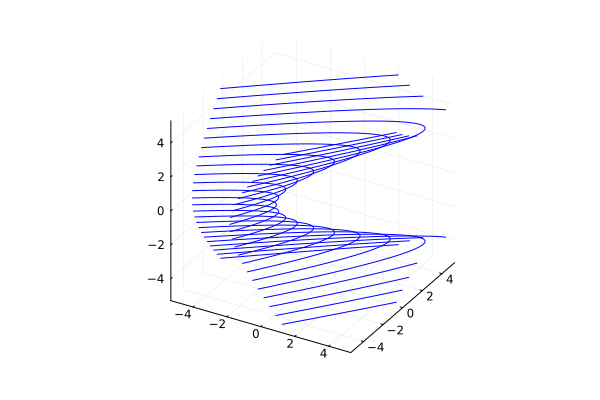
\includegraphics[scale=0.5]{Pictures/473.png}
\end{center}

\section{important expressions}
\begin{itemize}
    \item Tangent Planes:
    \begin{equation}
        \frac{\delta F}{\delta x}(x_0,y_0,z_0)(x-x_0) + \frac{\delta F}{\delta y}(x_0,y_0,z_0)(y-y_0) + \frac{\delta F}{\delta z}(x_0,y_0,z_0)(z-z_0) = 0 
    \end{equation}
    \item Directional Derivative:
    \begin{equation}
        \frac{d}{dt}f(x_0+tu,y_0+tu_z) | 0
    \end{equation}
\end{itemize}

\chapterimage{Heading4.jpg} % Chapter heading image

\chapter{Superior order derivatives}

\section{Taylor's Theorem}
let

$$ f: \mathbb{R} \to \mathbb{R} $$

Then:
\begin{equation}
    F(x) = F(a) + F'(a) (x-a) + \frac{F''(a)}{\alpha !} (x-a)^2 + \dots + \frac{F^{(k)}(x-a)^k}{k!} (x-a)^k + error    
\end{equation}

this can also be written as:
\begin{equation}
    \Delta F(t_0) = F(t_0+\Delta t) - F(t_0)
\end{equation}

Generally, we can assume that given a theorem from $\mathbb{R}^n \to \mathbb{R}^n$

\begin{gather}
    \vec{x_0} = \begin{pmatrix}
        x_1 \\
        . \\
        . \\
        . \\
        x_n
    \end{pmatrix} ,
    \vec{h} = \begin{pmatrix}
        h_1 \\
        . \\
        . \\
        . \\
        h_n
    \end{pmatrix} \text{then:} \\
    f(\vec{x_0}+ \vec{h}) = f(\vec{x}_0) + \sum_{1}^{n} \frac{\delta f}{\delta x_i}(\vec{x_0}) + \frac{1}{2!} \sum_{i,j = 1}^{n} h_i h_j \frac{\delta^2 f}{\delta x_i \delta x_j} \vec{x_0} +  
    \frac{1}{3!} \sum_{i,j,k = 1}^{n} h_i h_j h_k \frac{\delta^3 f}{\delta x_i \delta x_j \delta x_k} \vec{x_0} + \dots 
\end{gather}

...That being said, we can mostly just stay with two. Triple derivatives are sure as hell weird. 

\section{Function extremes with real values.}

Given a set 'D' that is bound if we can find a value R > 0 such as:
$$ D \subseteq x^2 + y^2 \leq R^2 $$
and:
$$ D \subseteq \mathbb{R}^2 \to \mathbb{R} $$



% Simply upload additional images Heading5.jpg, Heading6.jpg etc. into the pictures folder

% \chapterimage{Heading5.jpg}
% \chapter{Third Set of Questions}


%----------------------------------------------------------------------------------------
%	References
%----------------------------------------------------------------------------------------

\chapterimage{Heading4.jpg} % Chapter heading image

\bibliographystyle{plain} % Change this to IEEE or Harvard etc.
\bibliography{references}


\end{document}